I conducted two case studies that use PHMMs to model the behaviour and foraging success of eleven resident killer whales (nine northern, two southern) off the coast of British Columbia, Canada. These case studies were primarily intended to test the predictive performance of the PHMM and demonstrate the process of applying it to ecological data. However, I also perform these case studies for their ecological significance. As mentioned earlier, understanding killer whale foraging and successful prey capture has been a research focus for years, as differences in foraging success may explain why the southern resident killer whale population is doing poorly compared to the northern residents \citep{Noren:2011, Tennessen:2023}. Thus, the results from these case studies can help ecologists correctly predict foraging behaviours that are meaningful for conservation. 

%\subsection{Data Collection}

The data for these case studies were collected in August and September 2020 using a CATS time-depth recorder (TDR) from Customizable Animal Tracking Solutions (www.cats.is). All resident killer whales were tagged with suction-cup attached CATS tags off the coast of British Columbia. These tags were deployed using an adjustable 6-8 meter carbon fiber pole. Each tag was programmed to release within 3 to 24 hours of attachment. Post-deployment, the instruments were retrieved utilizing a combination of a Wildlife Computers 363C SPOT tag (providing Argos satellite positions), a goniometer, an ultra high frequency receiver, and a yagi antenna. The tags were equipped with an array of sensors, including 3D kinematic sensors (accelerometer, magnetometer, gyroscope), a time-depth recorder, a hydrophone, and a camera. All sensors were set to sample at a frequency of 50 Hz. Depth readings were calibrated using a MATLAB package developed by \citet{Cade:2021}, which allowed for the extraction of heading, pitch, and roll, as well as three-dimensional dynamic acceleration within the reference frame of the killer whale.

Using these data, I developed two PHMMs to identify killer whale foraging behaviours at different scales. The first PHMM estimated killer whale dive types using individual dives as observations, with some dives labelled using drone videos. The second PHMM estimated prey capture events using high-frequency biologging data as observations, with some observations labelled using video and audio recordings of prey capture. For both case studies, I modelled each killer whale as independent, but with shared parameters for their associated PHMMs. 

In both case studies, subject matter experts could identify labels with high confidence, so I defined $g^{(i)}$ according to Equation (\ref{eqn:g_perfect}). I also used $k$-fold cross-validation to calculate evaluation metrics in both case studies. In particular, I divided the data from all killer whales into $k$ folds, removed a fold from the original dataset, and fit the model using 10 random parameter initialization and a custom version of the momentuHMM package in \texttt{R} \citep{McClintock:2018, R:2023}. I then used the forward-backward algorithm on the held-out fold (while ignoring its true labels) to obtain estimated probabilities of each hidden state (dive phase or dive type). I repeated this process for each fold to obtain hidden state probability estimates for the entire data set.

\subsection{Case Study 1: Behavioural Classification of Killer Whale Dives}

For my first case study, I assigned a latent behaviour to every killer whale dive. To this end, I modelled the data from each killer whale as a sequence of dives and modelled each sequence with a PHMM. %Each PHMM was independent, and all PHMMs had identical parameters. 
The hidden Markov chain was a sequence of dive types and the observations were summary statistics of each dive. I used three well-known killer whale behaviours as possible dive types: resting, travelling, or foraging \citep{McRae:2024}. 

\subsubsection{Data Processing}

I defined a dive as any period in which the killer whale was below a depth of 0.5 meters for at least 30 seconds, which includes only biologically meaningful dives and excludes surface behaviours. In line with previous studies \citep{Barajas:2017, McRae:2024}, I summarized each dive with its maximum depth and total duration.  Formally, the observation associated with whale $s$ and dive $t$ was denoted as $y_{s,t} = (m_{s,t},d_{s,t})$, where $m_{s,t}$ corresponds to maximum depth in meters and $d_{s,t}$ corresponds to dive duration in seconds. This processes resulted in a time series of $S=11$ killer whales, who together performed a total of $T=2169$ dives.

Using drone videos, a subject matter expert visually identified three diving behaviours: resting, travelling, and foraging \citep[classification criteria are given in Table 2 of][]{McRae:2024}. Formally, the label associated with whale $s$ and dive $t$ was denoted as $z_{s,t} \in \{\emptyset,1,2,3\}$, where each value of $z_{s,t}$ corresponds to either no label (if $z_{s,t} = \emptyset$), resting (if $z_{s,t} = 1$), travelling (if $z_{s,t} = 2$), or foraging (if $z_{s,t} = 3$). This resulted in a total of $|\calT| = 106$ labels for dive types. 

\subsubsection{Model Formulation}

I used a PHMM with $N = 3$ dive types to match the drone-identified labels of resting, travelling, and foraging dives. For whale $s$ and dive $t$, I denoted the hidden dive type as $X_{s,t} \in \{1,2,3\}$. 
%
Histograms and scatter plots revealed that dive duration and maximum depth looked to be distributed approximately as mixtures of log-normal distributions, and the two features were also highly correlated. Therefore, I set the joint, state-dependent distribution of the observations to be a bi-variate log-normal distribution. 

Recall that I used thresholds of $m_{s,t} \geq 0.5$ and $d_{s,t} \geq 30$ to define biologically relevant dives. However, I modelled these observations using a two-dimensional log-normal distribution whose sample space is $\bbR_{>0}^2$, so my model is misspecified. I could use a truncated multivariate log-normal distribution instead, but many HMM software packages do not incorporate truncated log-normal distributions by default \citep{McClintock:2018,Visser:2010}, and several ecological studies make this modelling choice as well \citep{Barajas:2017, Quick:2017, Tennessen:2019b}. I therefore use a non-truncated log-normal distribution for simplicity and repeatability. %add something about the final model is still good.

Again, I model the killer whale dive profiles as independent from one another, but with shared parameters. Denote the observations from whale $s$ as $\bfy_s = \{y_{s,t}\}_{t=1}^{T_s}$ and the labels from whale $s$ as $\bfz_s = \{z_{s,t}\}_{t=1}^{T_s}$, where $T_s$ is the number of dives associated with whale $s$. Then, the total likelihood for the model with weight $\alpha$ and parameters $\bfdelta, \bfGamma, \bftheta$ and $\bfbeta$ is $\prod_{s=1}^{11} p_\alpha (\bfy_s,\bfz_s ~;~ \bfdelta, \bfGamma, \bftheta, \bfbeta)$, where $p_\alpha$ is defined in Equation (\ref{eqn:PHMM_like_alpha}).

\subsubsection{Model Selection and Evaluation}

I fit five different candidate PHMMs corresponding to five different values of $\alpha$. In line with the cross-validation procedure from Section 3, I tested $\alpha = 0$, which ignores all unlabelled data; $\alpha = 1$, which gives equal weight to all observations; and $\alpha = |\calT| / (T - |\calT|) = 0.049$, which approximately balances the contribution of labelled and unlabelled observations. For completeness, I also tested $\alpha = 0.025$, which averages $\alpha = 0$ and $\alpha = 0.049$; and $\alpha = 0.525$, which averages $\alpha = 0.049$ and $\alpha = 1$.

I randomly divided each killer whale dive profile into two ``sub-profiles" of contiguous dives such that both sub-profiles had an equal number of labels. The resulting 22 sub-profiles were used as folds in a cross-validation scheme to estimate the probability of each dive's type conditioned on the observations (i.e., $\bbP(X_{s,t} = i \mid \bfY_s = \bfy_s)$ for $s = 1,\ldots,11$; $t = 1,\ldots,T_s$; and $i = 1,2,3$). I then calculated the sensitivity, specificity, and area under the receiver operating characteristic curve (AUC) associated with identifying each dive type. Sensitivity is the proportion of dives that were observed to be a certain type that were correctly identified as that type (i.e. the true positive rate). Specificity is the proportion of dives that were observed to not be of a certain type that were correctly identified as not that type (i.e. the true negative rate). AUC balances sensitivity and specificity and usually takes values between 0 and 1, where higher is better \citep{Bradley:1997}. I also ran the Viterbi algorithm on each fold within the cross validation procedure and plotted the resulting dive profiles as a visual model evaluation tool \citep{Viterbi:1967}.

%A total of eight profiles had labelled dives, and I divided each into two sub-profiles to make a total of 16 sub-profiles. I randomly divided each killer whale's dive profile in two such that there were an equal number of labels on both sub-profiles. For each value of $\alpha$, I fit the PHMM 16 times, leaving out one of the sub-profiles for each of the 16 analyses. For each fold, I used 10 random parameter initializations and fit the PHMM models on Compute Canada Cedar nodes with 8GB of RAM. The 10 parameter initializations did not depend upon the value of $\alpha$. Fitting was done in $\texttt{R}$ using the momentuHMM package for model formulation and the nlm package for optimization \citep{McClintock:2018,R:2023}. I then selected the PHMM with the maximum likelihood of the 10 random parameter initializations. Next, I removed the labels on the held-out sub-profiles and used the corresponding PHMM fits to predict dive types. I predicted the dive types using the forward-backward algorithm \citep{Zucchini:2016}. This procedure gave us estimated probabilities of each dive type for all labelled dives across the 16 held-out sub-profiles. 

\subsubsection{Results}

The PHMMs with $\alpha \in (0,1)$ tended to obtain better results for cross-validated sensitivity, specificity, and AUC, demonstrating the effectiveness of my weighted likelihood approach (Figure \ref{fig:sens_spec}). Compared to the PHMMs with $\alpha = 0$ and $\alpha = 1$, the PHMM with $\alpha = 0.049$ had the best sensitivity for foraging dives and travelling dives, and it had the second-best sensitivity for resting dives. It had the best specificity for resting dives and travelling dives, and its specificity for foraging dives was comparable to the other models. In addition, the PHMM with $\alpha = 0.049$ had an AUC for resting that was comparable or better than the other PHMMs (0.866), but it had the best AUC for foraging (0.955) and the best AUC for travelling (0.926). Results for the PHMMs with $\alpha = 0.025$ and $\alpha = 0.525$ are similar to the PHMM with $\alpha = 0.049$ (see Appendix). 

\begin{figure}
    \centering
    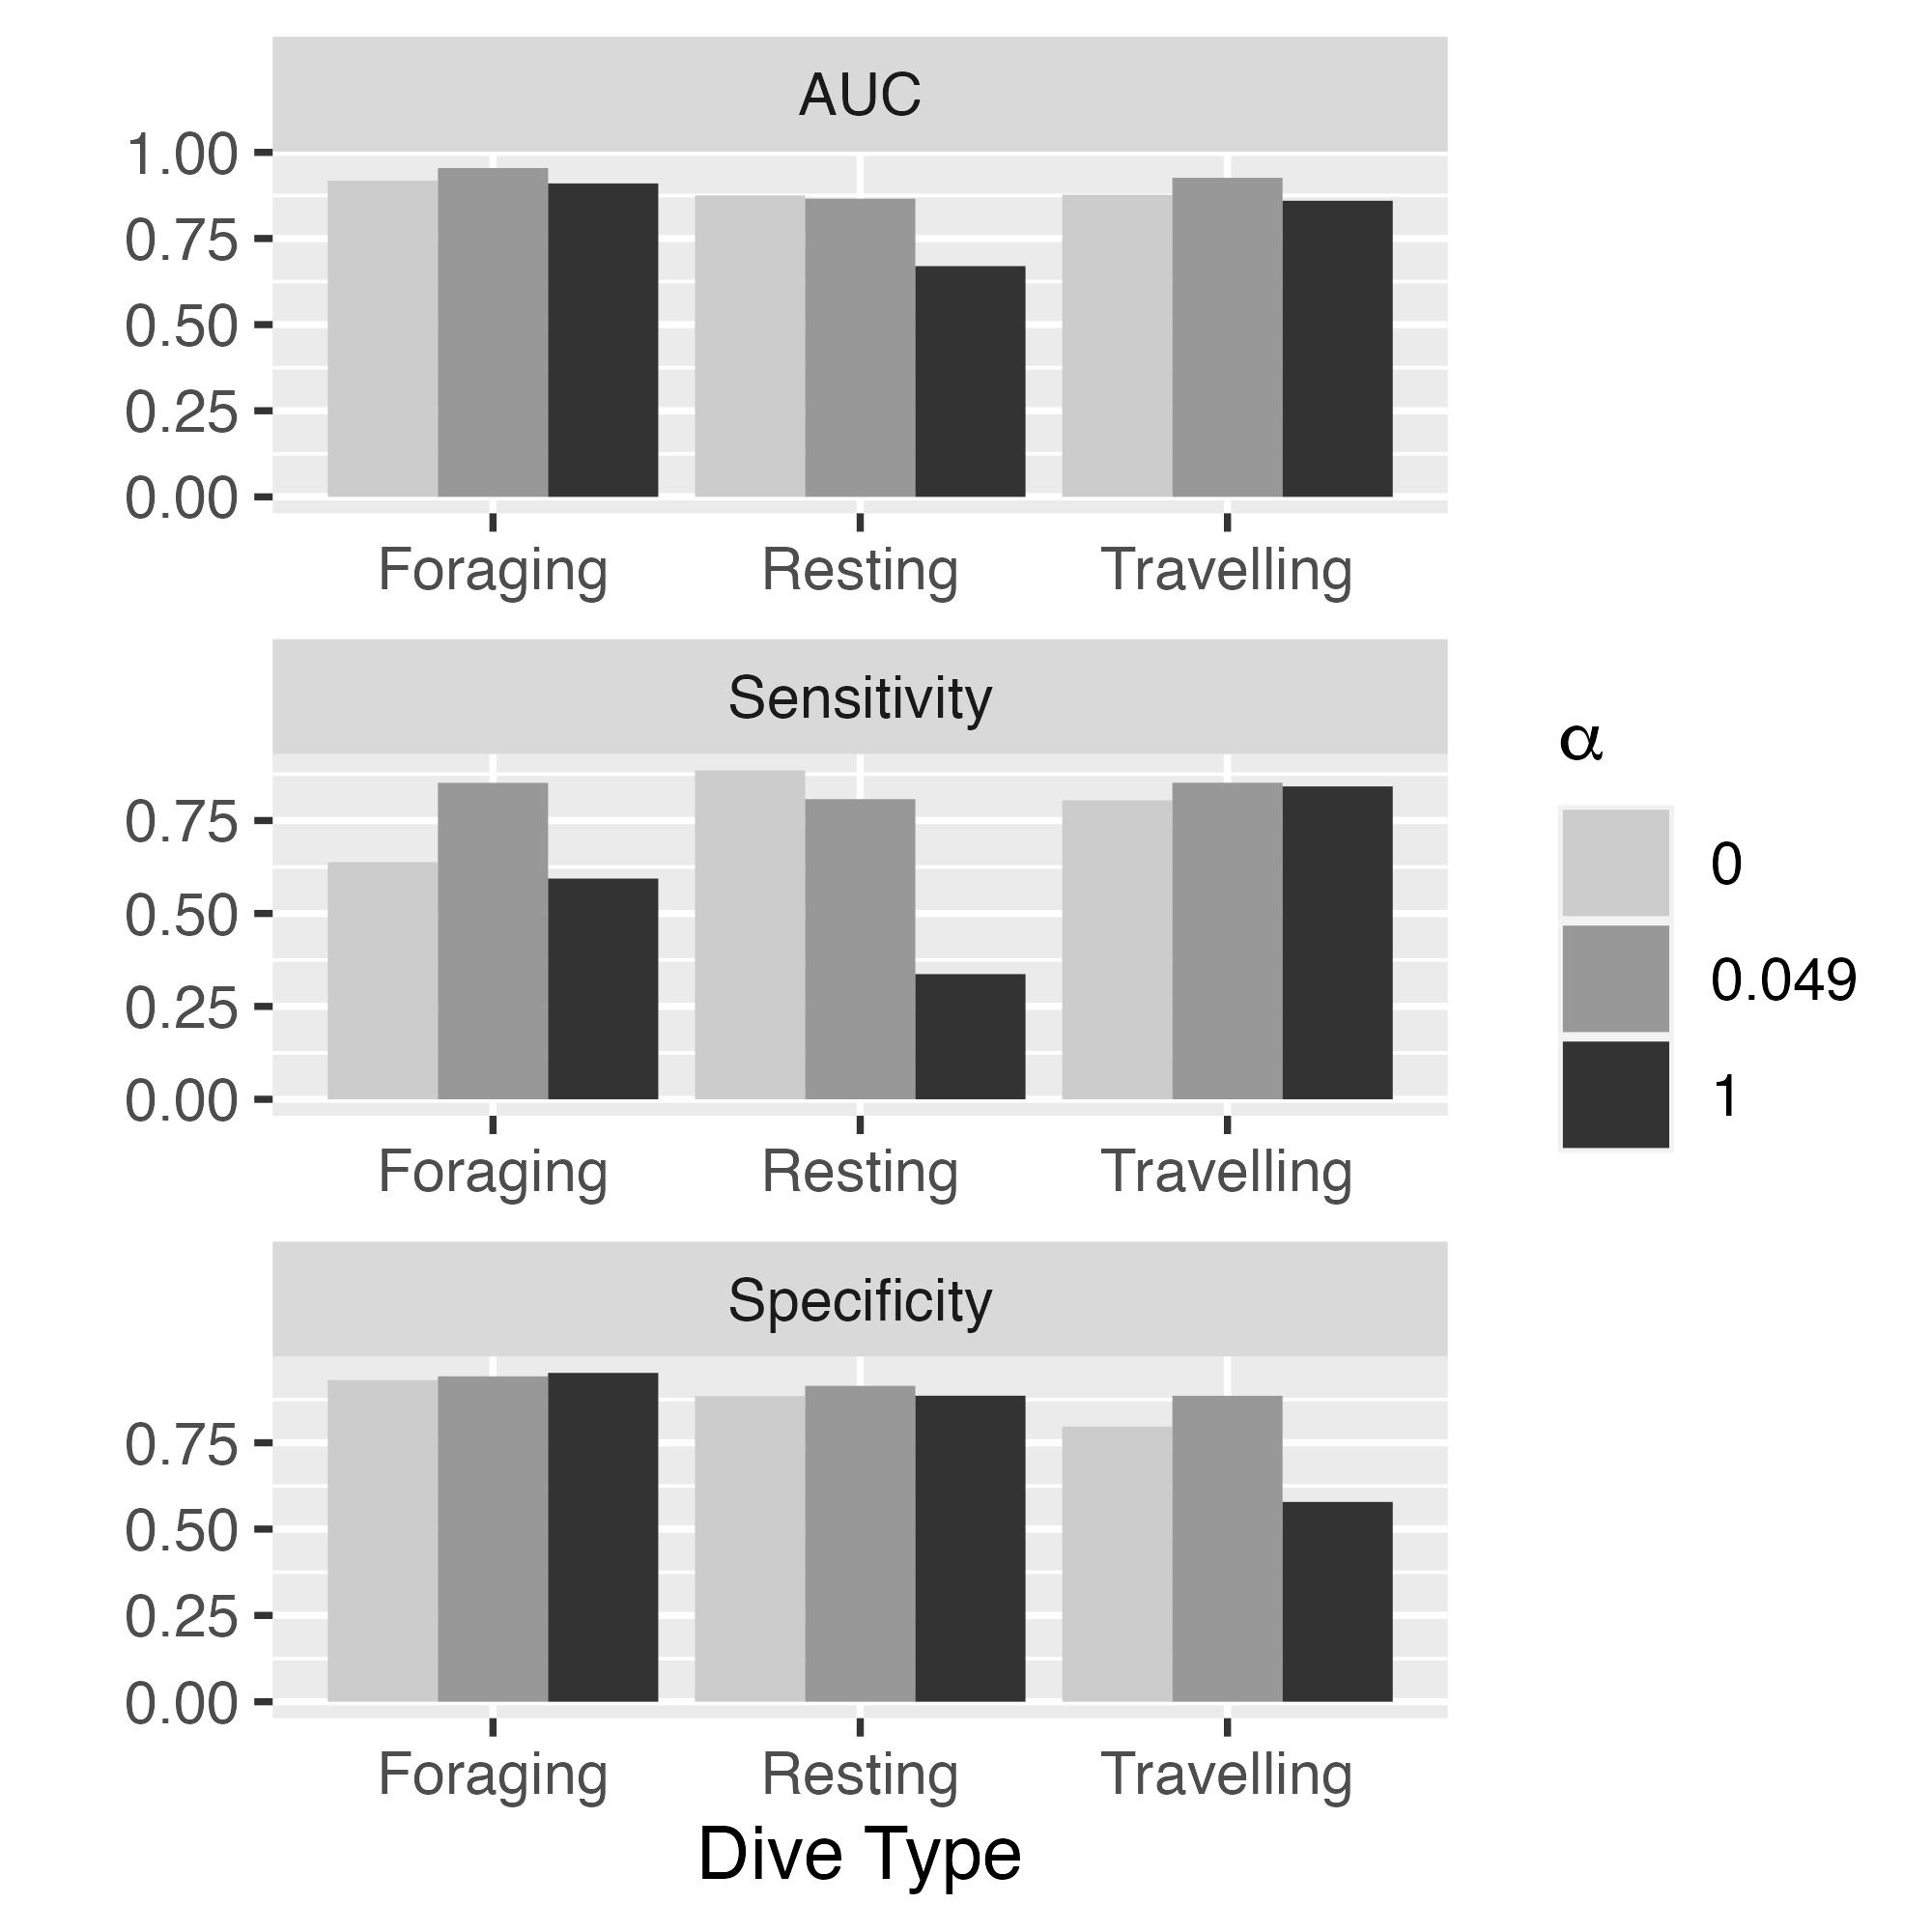
\includegraphics[width=4in]{plt/1-1-1-logMDDD_all_model_comparison.png}
    \caption{Sensitivity, specificity, and AUC values associated with each dive type. True values are determined via the drone-detected dive types. The PHMMs for each value of $\alpha$ were fit using the entire dataset with a selected sub-profile held out. Then, the dives for that sub-profile were estimated by using the forward-backward algorithm on the sub-profile with the drone-detected labels removed. I repeated this process for every sub-profile to get a full set of estimated dive types. Results for PHMMs with $\alpha = 0.025$ and $\alpha = 0.525$ are in the Appendix.}
    \label{fig:sens_spec}
\end{figure}

The PHMMs with $\alpha \in (0,1)$ were also more biologically interpretable compared to those with $\alpha = 0$ and $\alpha = 1$. Namely, for the PHMMs with $\alpha \in (0,1)$, the time series of decoded dive types contained long sequences of a single dive type (Figure \ref{fig:viterbi_dives_D26b}). This behaviour matches prior studies that model killer whale behaviours as lasting for tens of minutes to hours \citep{McRae:2024}. In comparison, the PHMM with $\alpha = 1$ resulted in a dive profile that switched relatively frequently between foraging and resting dives (e.g., Figure \ref{fig:viterbi_dives_D26b}a). The PHMM with $\alpha = 0$ produced better results than the PHMM with $\alpha = 1$, but it still estimated some rapidly switching dive types (e.g., Figure \ref{fig:viterbi_dives_D26b}c).

%The cross-validation demonstrated that the best alpha for detecting foraging according to AUC and sensitivity was 0.049 (Fig 3., Supp Material that has the other values of alpha). This alpha value also provided the most sensible decoding of the states (Fig 4).

%The PHMM that placed equal weight on labelled and unlabelled dives ($\alpha = 1$) resulted in a dive profile that switched relatively frequently between foraging and resting dives (e.g., Figure \ref{fig:viterbi_dives_D26b}a). This behaviour is inconsistent with prior studies, as these killer whale dive types are usually modelled as lasting for several dives over the coarse of tens of minutes to hours \citep{McRae:2024}. In terms of classification accuracy, the PHMM with $\alpha = 1$ misclassified all of the drone-labelled resting dives as foraging dives and labelled the true travelling dive about 30 minutes into the dive profile as a resting dive (see Figure \ref{fig:viterbi_dives_D26b}a). Of the 5 values of $\alpha$, the PHMM with $\alpha = 1$ had the lowest sensitivity associated with resting and foraging and the lowest specificity associated with travelling (Figure \ref{fig:sens_spec}). In addition, the PHMM with $\alpha = 1$ had the worst AUC values for foraging (0.910), resting (0.670), and travelling (0.860) compared to models with other values of $\alpha$.

\begin{figure}
    \centering
    \begin{subfigure}[t]{0.45\textwidth}
        \centering
        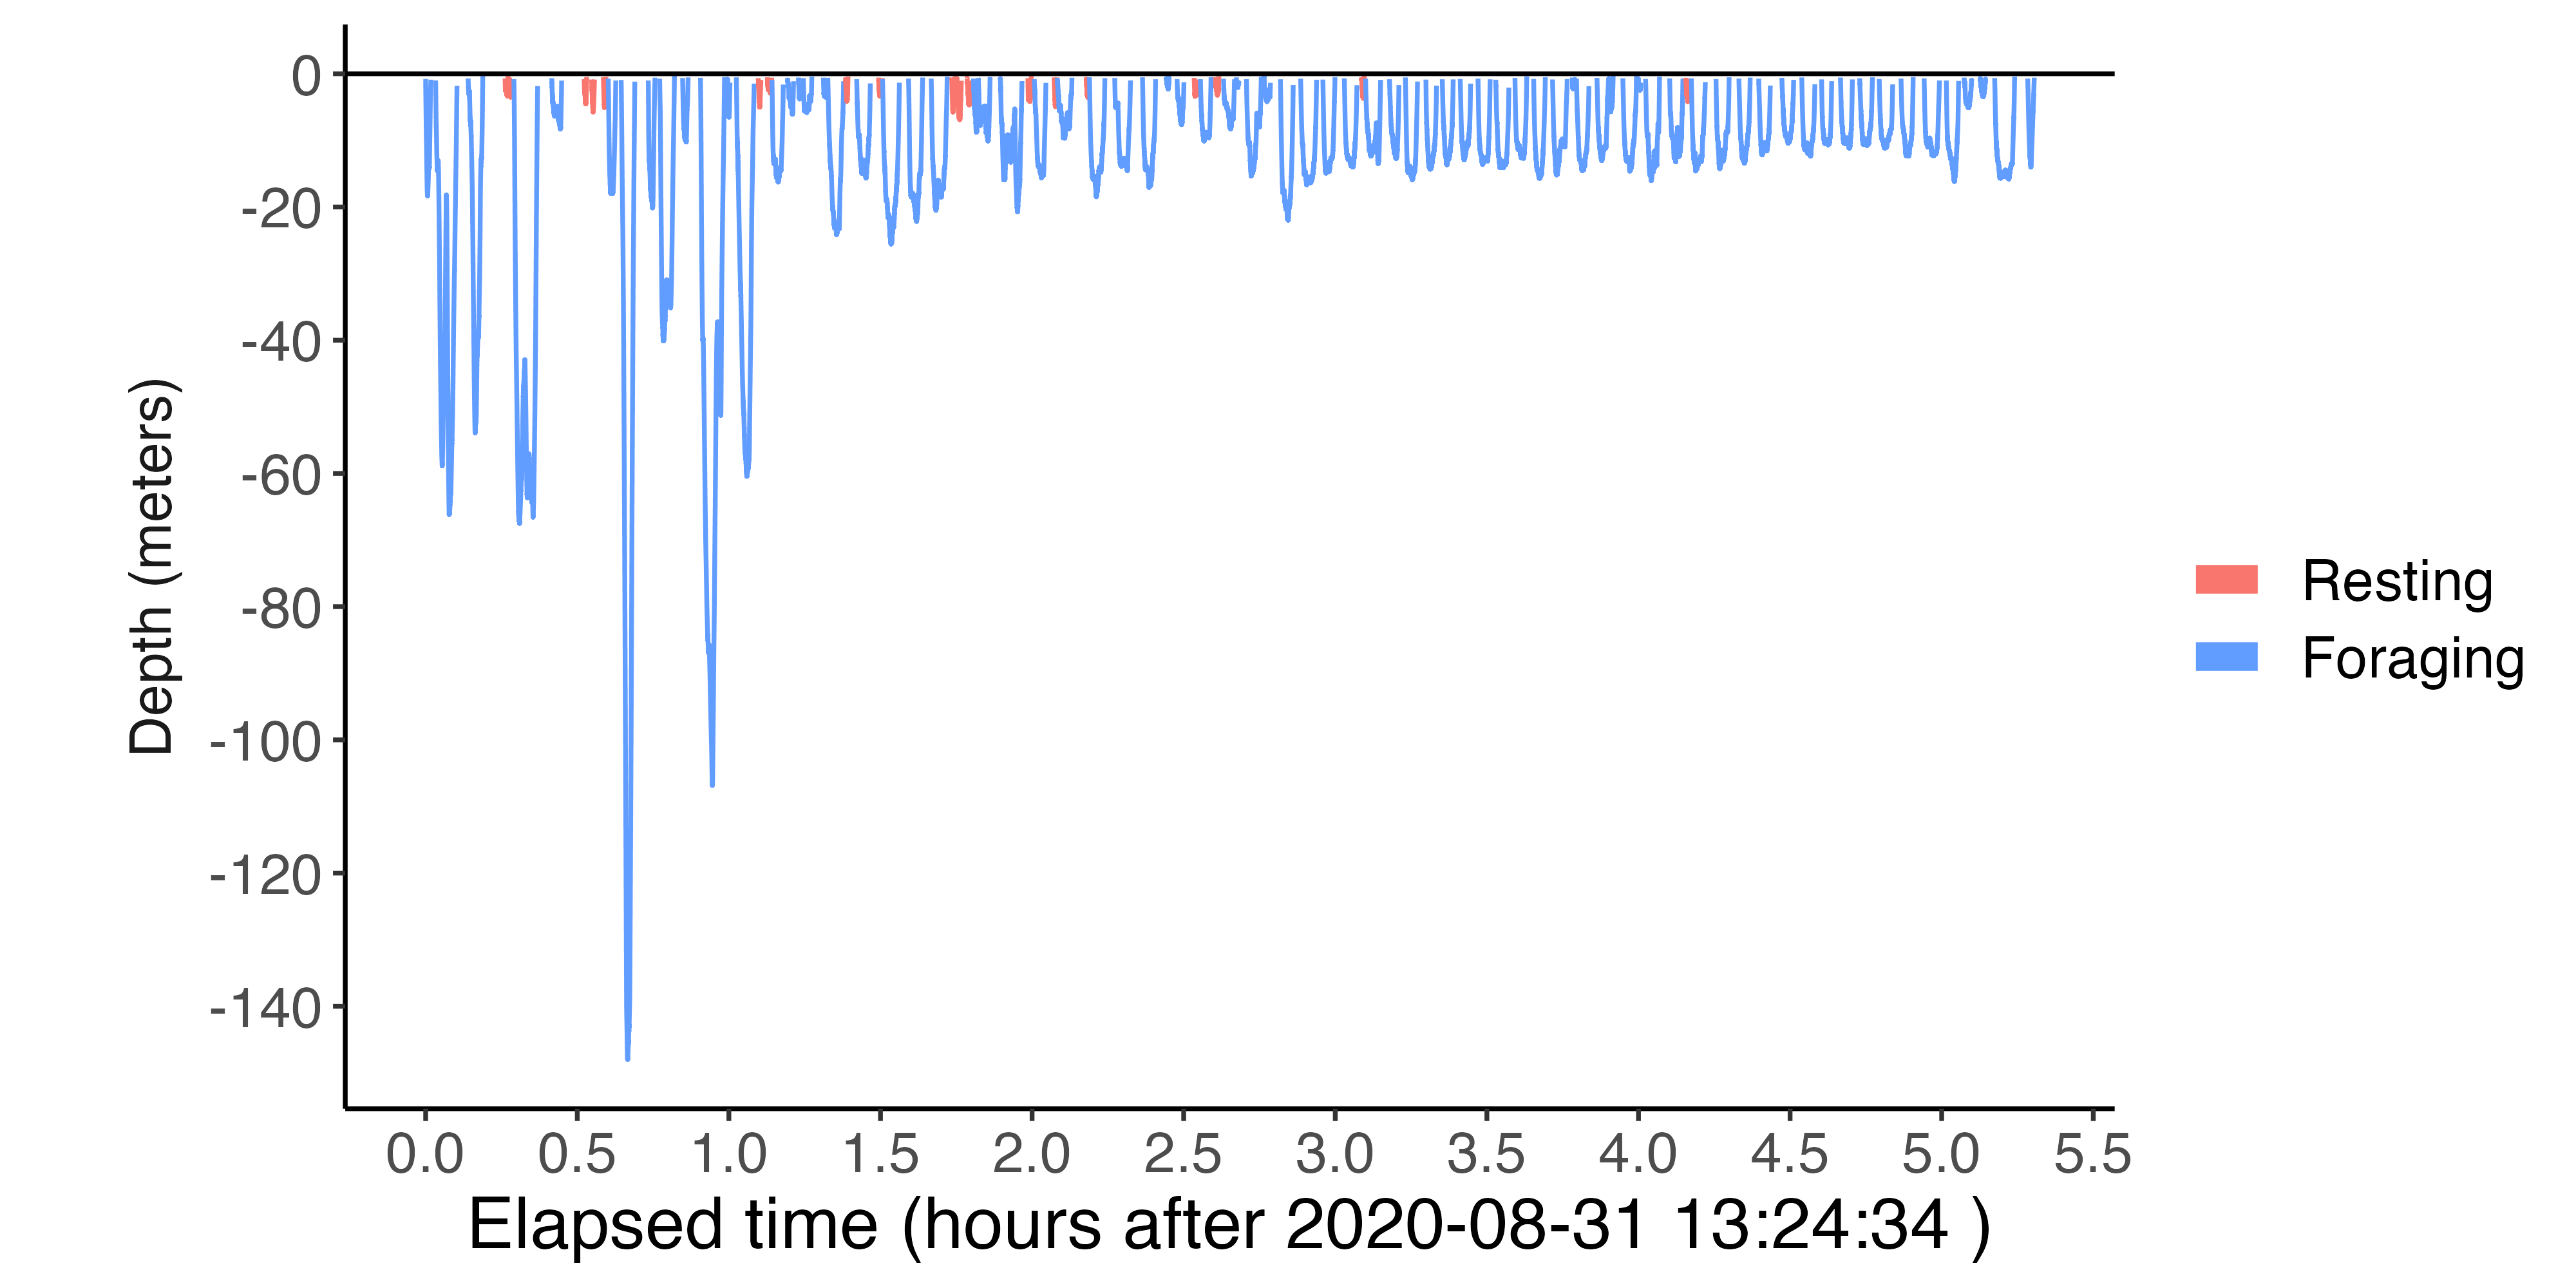
\includegraphics[width = 3in]{plt/D26b-profile-D26b-fixed-1.png}
        \caption{Decoded dives for PHMM with $\alpha = 1.000$ (the ``natural" weighting).}
    \end{subfigure}%
    ~ 
    \begin{subfigure}[t]{0.45\textwidth}
        \centering
        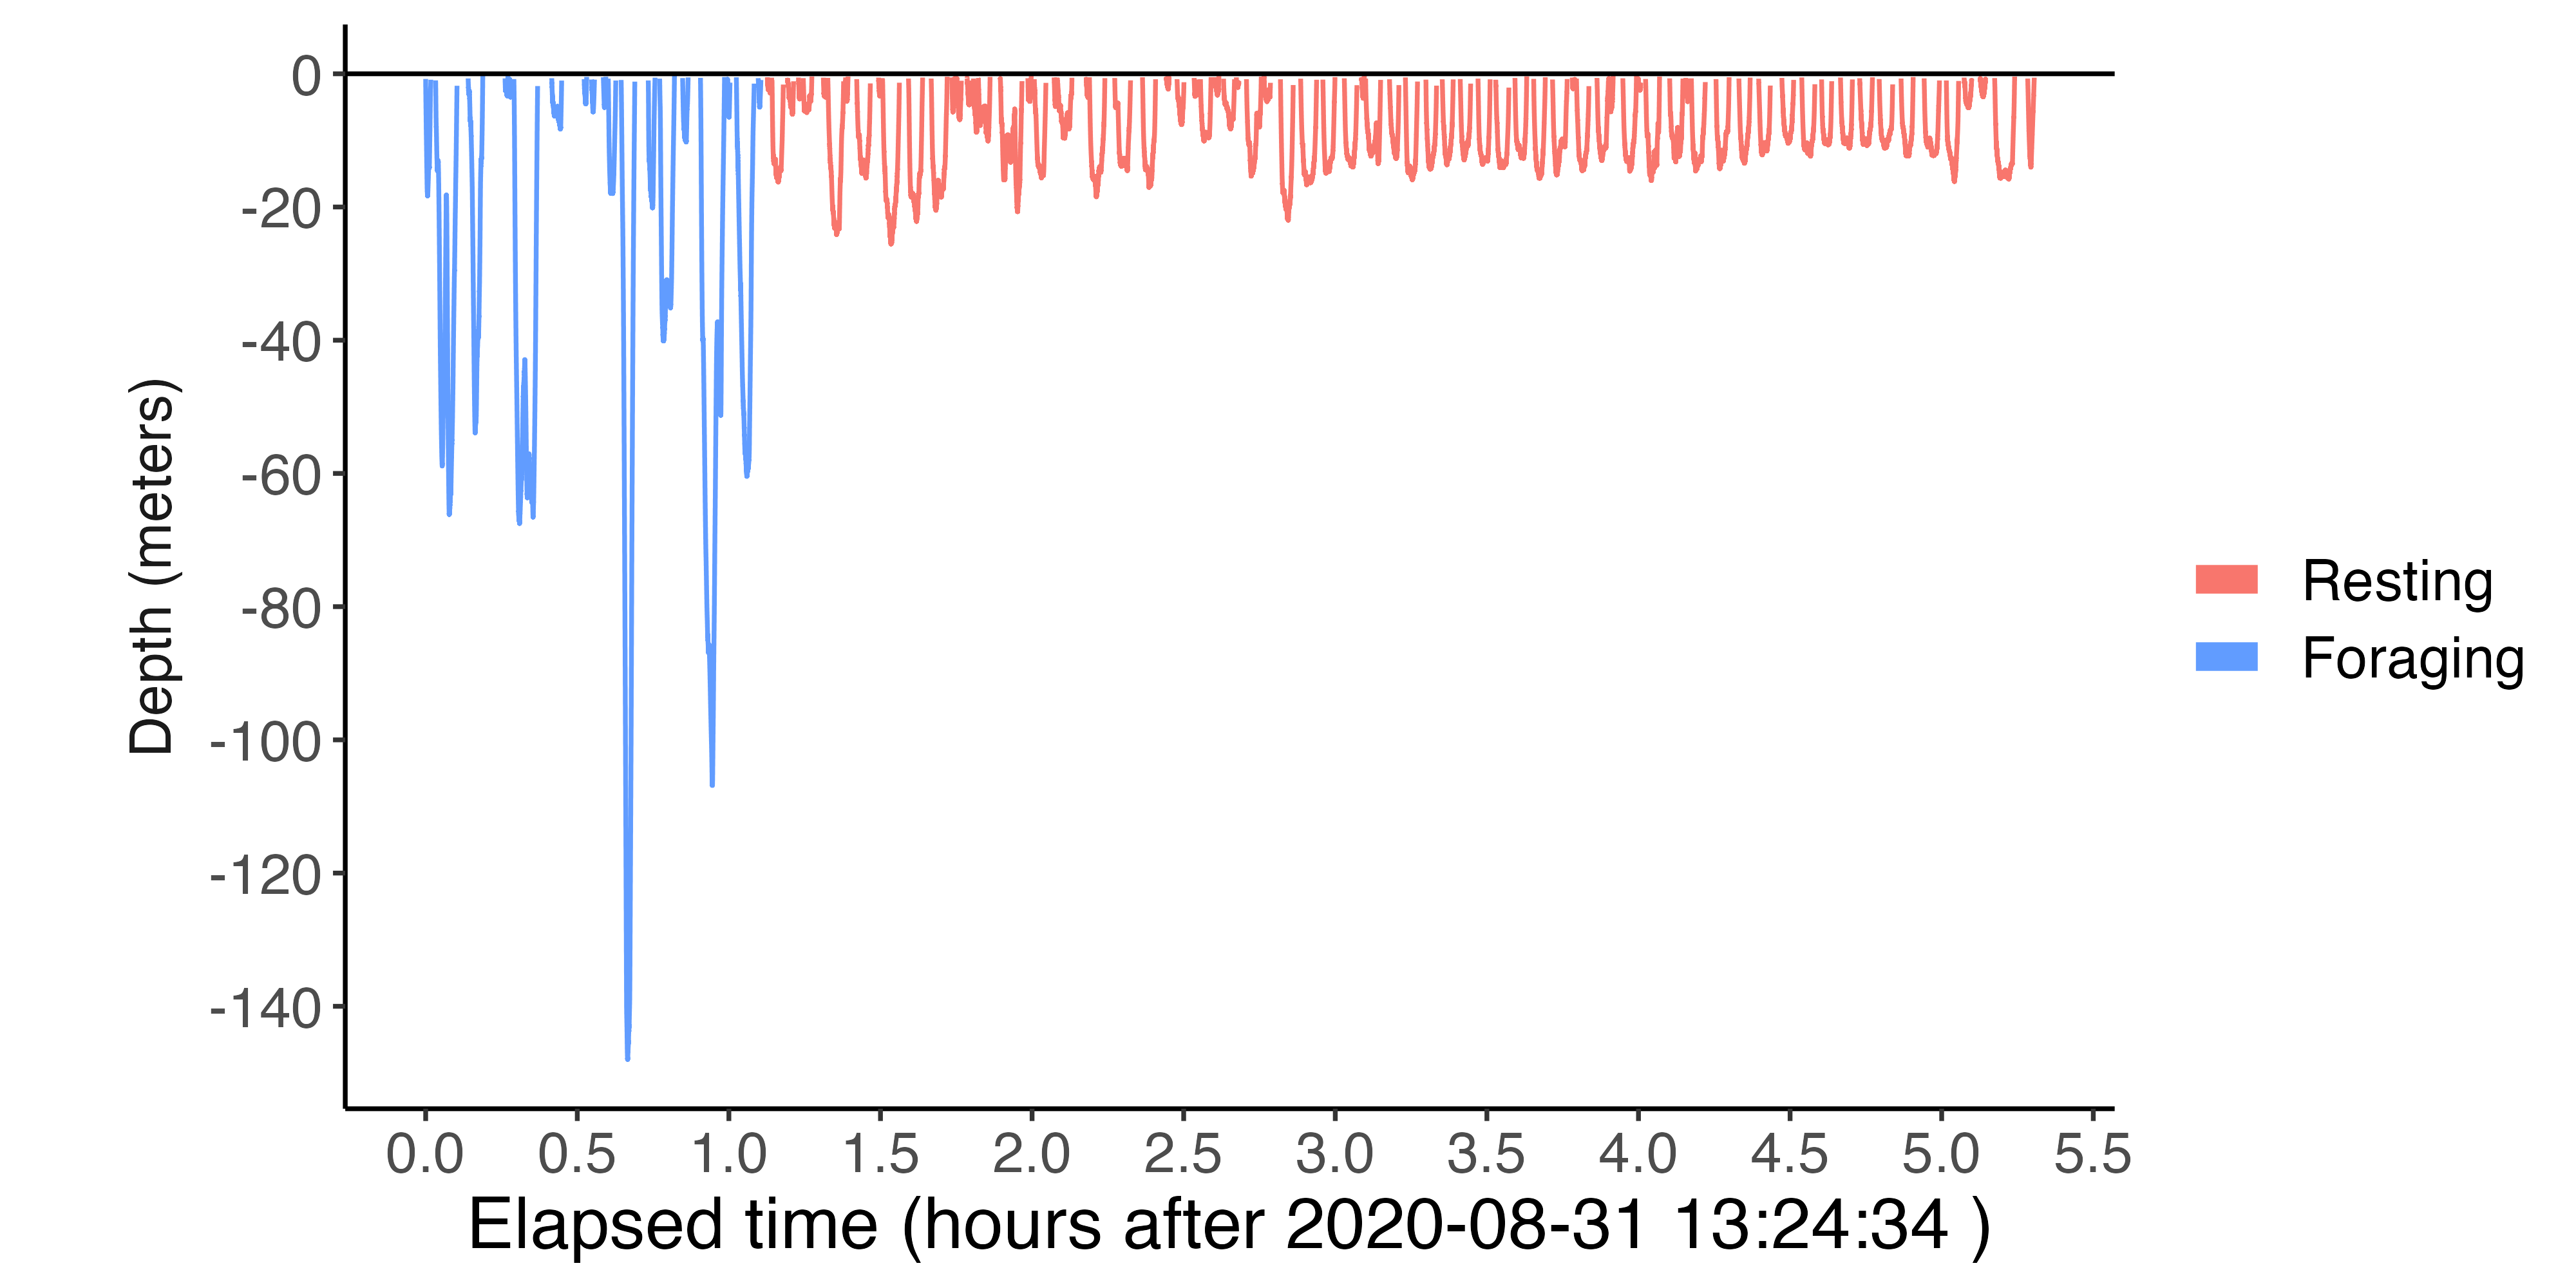
\includegraphics[width = 3in]{plt/D26b-profile-D26b-fixed-0.049.png}
        \caption{Decoded dives for PHMM with $\alpha = 0.049$.}
    \end{subfigure}
    \\
    \begin{subfigure}[t]{0.45\textwidth}
        \centering
        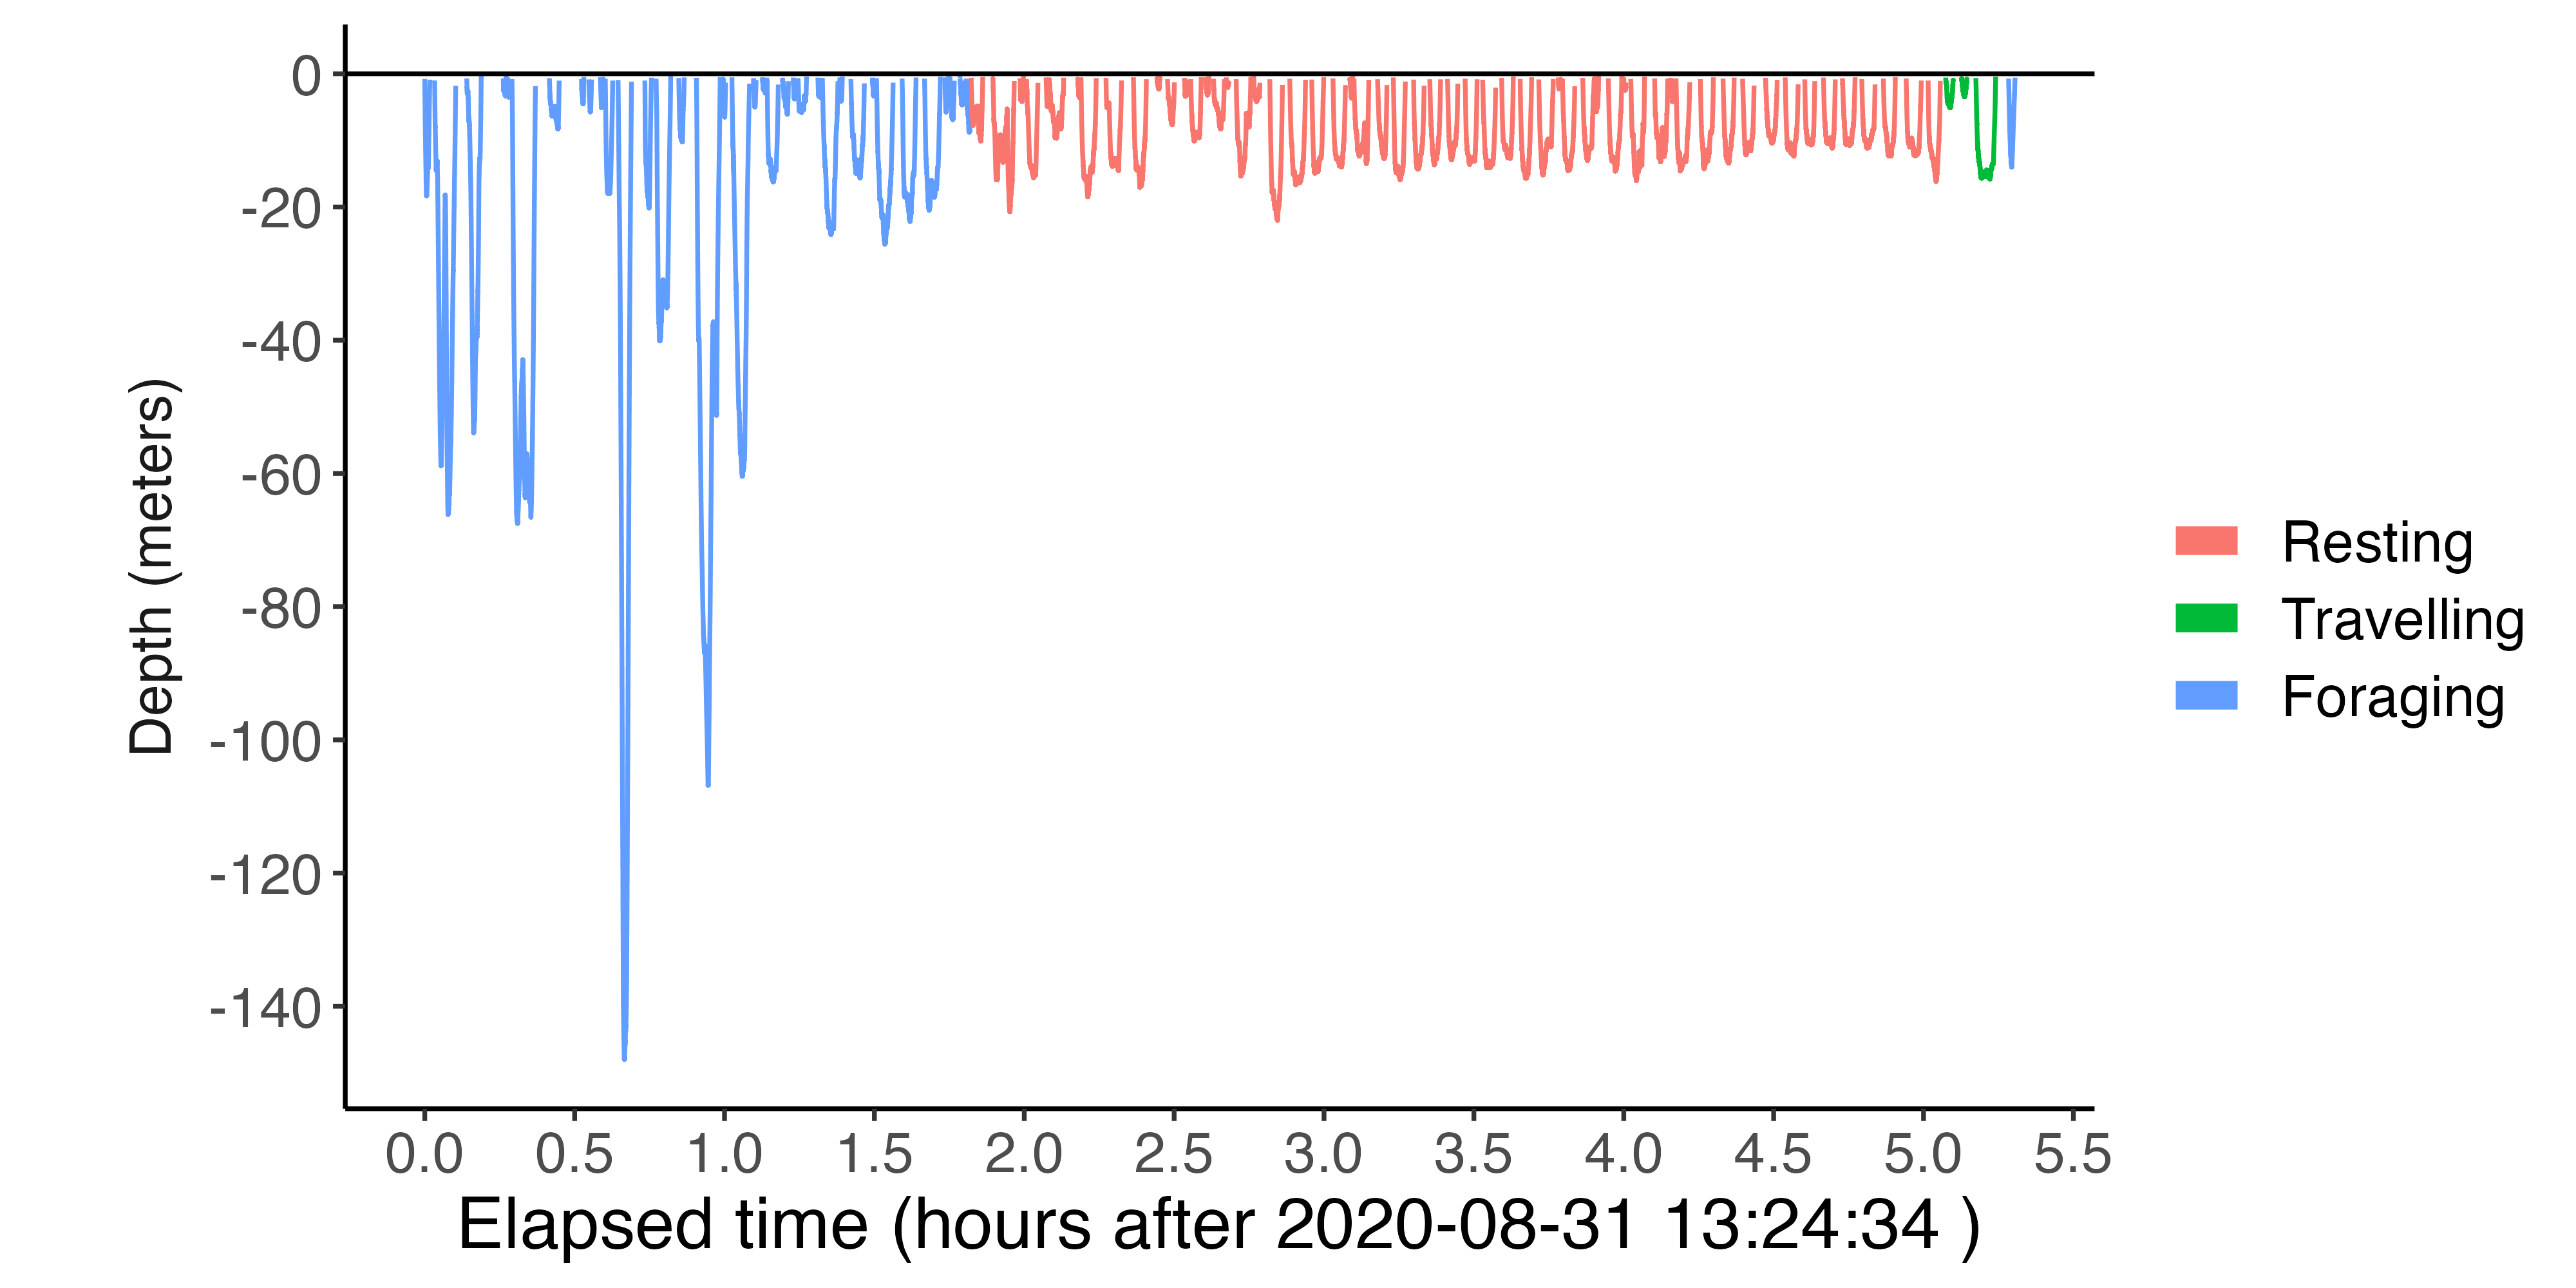
\includegraphics[width = 3in]{plt/D26b-profile-D26b-fixed-0.png}
        \caption{Decoded dives for PHMM with $\alpha = 0.000$ (treating the unlabelled observations as missing).}
    \end{subfigure}
    ~
    \begin{subfigure}[t]{0.45\textwidth}
        \centering
        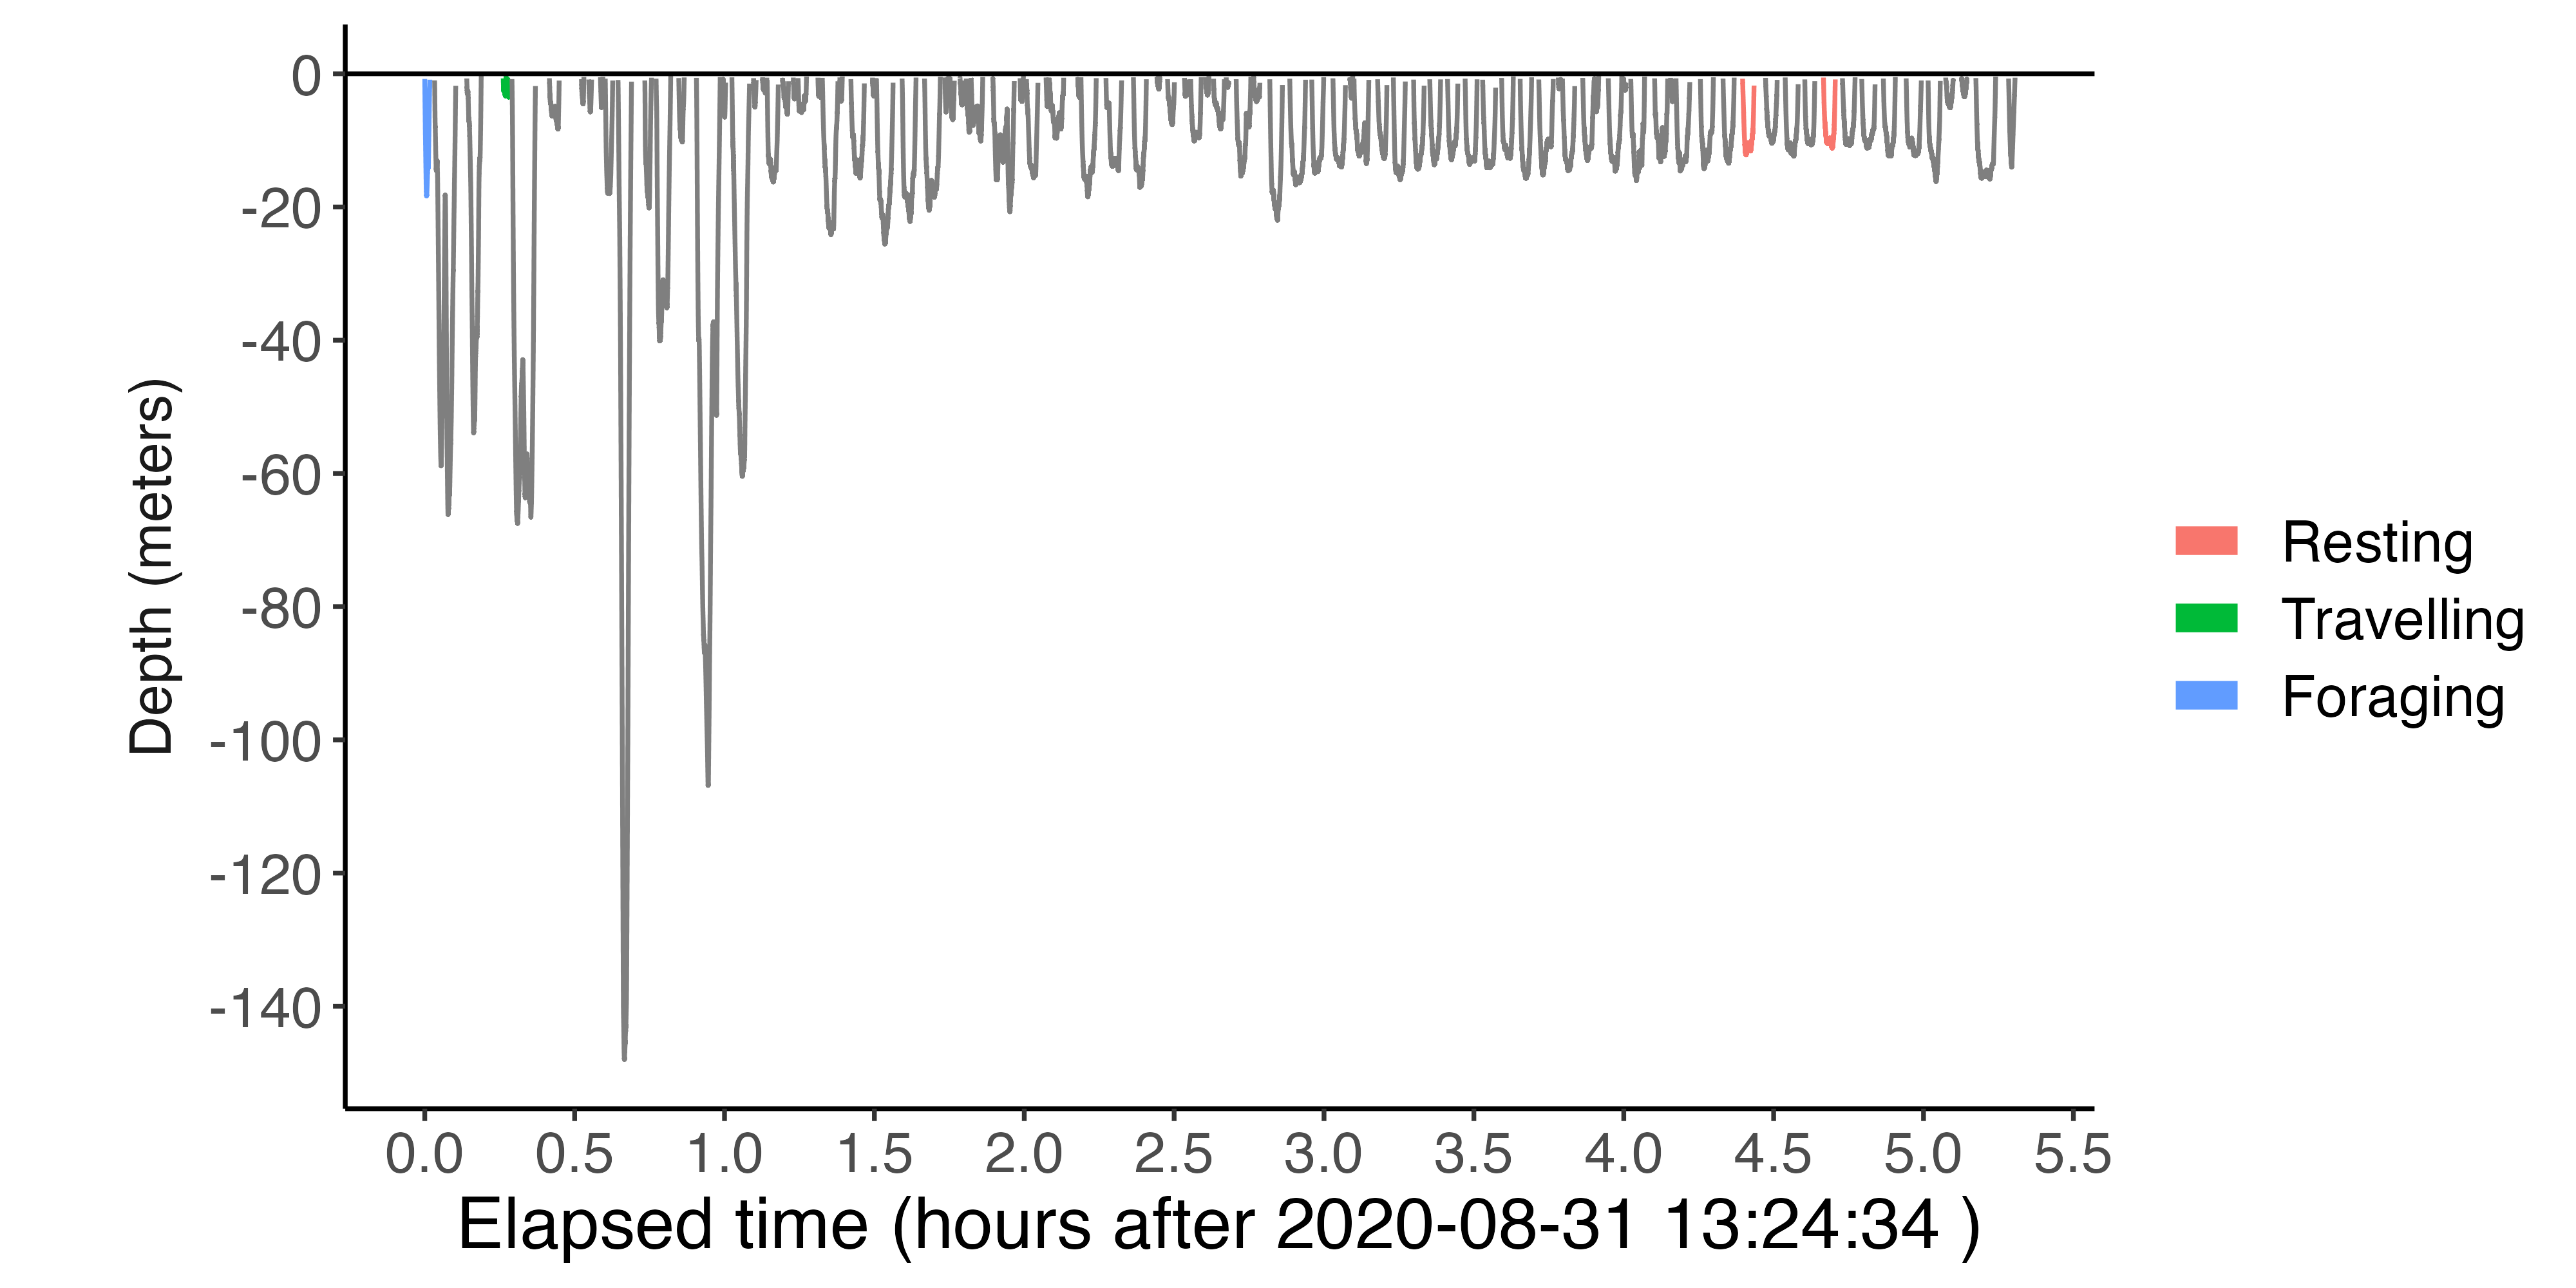
\includegraphics[width = 3in]{plt/D26b-profile-D26b-known_states.png}
        \caption{Dive profile with true drone-detected labels.}
    \end{subfigure}
    \caption{Viterbi-decoded dives for a given sub-profile and several different PHMMs. Each PHMM was fit to the dataset with the sub-profile held out. Then the Viterbi algorithm was used on the held-out dataset with its labels removed in order to test the predictive performance of each PHMM.}
    \label{fig:viterbi_dives_D26b}
\end{figure}

The PHMM that completely ignored unlabelled dives ($\alpha = 0$) obtained better results than the PHMM that fully included the unlabelled dives ($\alpha = 1$). While one may expect that more data should improve accuracy, including unlabelled data is known to degrade the performance of a classifier in certain situations \citep{Singh:2008}. It is thus natural that the optimal approach for this case study neither fully included nor totally ignored the labelled dive types. %For the selected sub-profile, this PHMM showed less sudden switching between dive types than the PHMM with $\alpha = 1$. It also correctly labelled the drone-detected dives with the exception of the travelling dive around 30 minutes into the dive profile (Figure \ref{fig:viterbi_dives_D26b}). It had the highest sensitivity for resting dives, but the lowest sensitivity for travelling dives and the second lowest sensitivity for foraging dives. It had noticeably lower specificity for travelling dives compared to the PHMMs with $\alpha = 0.025$ and $\alpha = 0.049$ (Figure \ref{fig:sens_spec}). In addition, the PHMM with $\alpha = 0$ had the best AUC value for resting (0.875) and the second-best AUC values for foraging (0.918) and travelling (0.877) compared to the other values of $\alpha$.

%These results indicate that the natural weighting currently used by practitioners ($\alpha = 1$) is not always optimal. Surprisingly, completely ignoring unlabelled observations can improve classification performance, even though it corresponds to ignoring $\approx 95\%$ of the data in this case study. However, I found that the best option was to adopt a hybrid approach, down-weight the unlabelled observations, and tune the weighting parameter using cross validation.

Finally, I used the PHMM with $\alpha = 0.049$ to estimate how often the northern and southern resident killer whales engaged in foraging behaviour. In particular, I fit the PHMM to the entire data set, including all labels, and then ran the forward-backward algorithm on all whales and dives to calculate $\bbP(X_{s,t} = 3 \mid \bfY_s)$ for $t = 1,\ldots,T_s$ and $s = 1,\ldots,11$. Then, I labelled dive $t$ of whale $s$ as foraging if its decoded probability of foraging was above 50\%. Using this procedure, I estimated that southern resident killer whales foraged for 5.47 hours, or 32.0\% of the time, and that northern residents foraged for 17.90 hours, or 26.8\% of the time. This sample size was very small (2 southern residents and 9 northern residents), but these results are consistent with \citet{Tennessen:2023}, who found that southern residents spent less time travelling and resting compared to the northern residents.